\documentclass[tikz]{standalone}

\begin{document}

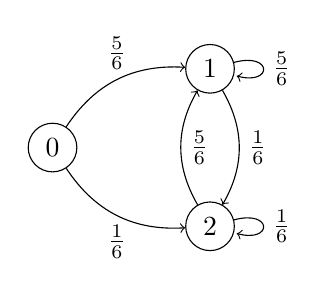
\begin{tikzpicture}
    \node [circle , draw ] (zero) at (0,0) {$0$};
    \node [circle , draw ] (one) at (2,1) {$1$};
    \node [circle , draw ] (two) at (2,-1) {$2$};
 
  \path[->] (one) edge [loop right] node {$\frac{5}{6}$} (one);
  \path[->] (two) edge [loop right] node {$\frac{1}{6}$} (two);
  \path[->] (zero) edge [bend left] node [above] {$\frac{5}{6}$} (one);
 \path[->] (zero) edge [bend right] node [below] {$\frac{1}{6}$} (two);
 \path[->] (one) edge [bend left] node [right] {$\frac{1}{6}$} (two);
 \path[->] (two) edge [bend left] node [right] {$\frac{5}{6}$} (one);
\end{tikzpicture}
\end{document}